\section*{Informations générales}
 
\begin{table}[H]
\centering
	\begin{tabularx}{16.8cm}{|X|X|}
	\hline
	\rowcolor{gray!40} Numéro du risque & Type du risque \\
	\hline
	005 & Mauvaise plannification \\
	\hline
	\end{tabularx}
\end{table}

\begin{table}[H]
\centering
	\begin{tabularx}{16.8cm}{|X|X|X|}
	\hline
	\rowcolor{gray!40} Date & Visa du \RQ & Visa du \CP \\
	\hline
	 28/01/2016 & pgpic & pgpic \\
	\hline
	\end{tabularx}
\end{table}

\begin{table}[H]
\centering
	\begin{tabularx}{16.8cm}{|X|X|X|X|}
	\hline
	\rowcolor{gray!40} Pilote & Activité WBS & Compte WBS & Phase d'apparition \\
	\hline
	 \Florian & Suivre les Risques et Opportunités & 1.2.3.2 & À partir du début du projet\\
	\hline
	\end{tabularx}
\end{table}

\section*{Description du risque}

\subsection*{Résumé}
	La mauvaise planification concerne principalement l’appréciation des délais des tâches et peut être expliquée par l’inexpérience du Chef PIC. Elle peut entrainer des retards de livraison des lots.

\subsection*{Analyse des causes}
	voir figure \ref{risque perte de document}.

\subsection*{Criticité}

\begin{table}[H]
\centering
	\begin{tabularx}{16.8cm}{|>{\columncolor{gray!40}}X|X|}
	\hline
	Gravité & 3\\
	\hline
	Probabilité & 2\\
	\hline
	Criticité & A surveiller\\
	\hline
	\end{tabularx}
\end{table}
\newpage

\section*{Actions}
\subsection*{Actions préventives}

\centering
	\begin{longtable}{|p{7cm}|p{7cm}|}
	\hline
	\rowcolor{gray!40} Numéro de cause & Actions préventives \\
	\hline
	1 & \begin{itemize}
		\item Formation au logiciel PGPIC.
                \item Mise en place de mêlées quotidiennes.
		\end{itemize} \\
	\hline
	2 & \begin{itemize}
		\item Le \CPACourt{} doit se tenir au courant des actions du CPCourt{}.
		\end{itemize} \\
	\hline
	\end{longtable}

\section*{Décision de clôture}
Par le \CP{} et le pilote du risque.
\begin{table}[H]
\centering
	\begin{tabularx}{16.8cm}{|X|X|}
	\hline
	\rowcolor{gray!40} Date de clôture & Raison de la clôture \\
	\hline
	  & \\
	\hline
	\end{tabularx}
\end{table}

\section*{Historique des modifications}
\begin{table}[H]
\centering
	\begin{tabularx}{16.8cm}{|X|X|}
	\hline
	Date & Modification \\
	\hline
	  & \\
	\hline
	\end{tabularx}
\end{table}
\newpage

\begin{landscape}
\begin{figure}
	\centering
	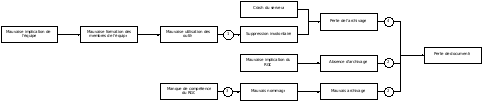
\includegraphics[scale=0.35]{images/AnalyseRisque_nPourquoi_FDR007.png}
	\caption{\label{risque perte de document}risque mauvaise plannification - méthode des n pourquoi}
\end{figure}
\end{landscape}
